\section{Stability}
\subsection{Method}
\begin{frame}{Principle}
\begin{itemize}
\item Stable direct integration scheme:
\begin{equation*}
\exists h_0 > 0 \hspace{0.5cm}\text{such as} \hspace{0.5cm} \forall h \in [0,h_0]
\end{equation*}  
a finite perturbation of the state vector at $t_n$ gives a non increasing variation of the state vector at a subsequent time $t_{n+j}$.
\item Initial distrubance:
\begin{equation}
\delta X_0 = X_0^\prime - X_0
\end{equation}
\item The non-perturbed solution:
\begin{align}
X_{n+1} &= H X_n + g_{n+1} \\
&= H^2 X_{n-1} + Hg_n + g_{n+1} \\
&\vdots\\
&= H^{n+1}X_0 + \sum^{n+1}_{j=0} H^{n-j+1}g_j
\end{align}
\end{itemize}
\end{frame}

\begin{frame}
\begin{itemize}
\item Perturbed solution:
\begin{equation}
X^\prime_{n+1} = H^{n+1}X_0^\prime + \sum^{n+1}_{j=0} H^{n-j+1}g_j
\end{equation}
\item Effect of initial disturbance at time $t_{n+1}$:
\begin{equation}
\delta X_{n+1} = H^{n+1} \delta X_0
\end{equation}
\item Associated eigenvalue problem :
\begin{equation}
det(H-\lambda I) = 0
\end{equation}
\item $\lambda_r, x_{(r)}$ associated eigenvalues and eigevectors.
\end{itemize}
\end{frame}
\begin{frame}
\begin{itemize}
\item Modal expension:
\begin{equation}
\delta X_0 = \sum^{2N}_{s=1} a_s x_{(s)}
\end{equation}
\item Transform the recurrence relation to:
\begin{align}
\delta X_{n+1} &= H^{n+1} \sum^{2N}_{s=1} a_s x_{(s)} \\
&= \sum^{2N}_{s=1} a_s \lambda_s^{n+1} x_{(s)}
\end{align} 
\item Disturbance will be amplified if eigenvalues are higher than unity.
\end{itemize}
\end{frame}

\begin{frame}
\begin{itemize}
\item Equation of motion at time $t_{n}$ and $t_{n+1}$:
\begin{equation}
\begin{cases}
    M  \Ddot{U}^n = -C \Dot{U}^n - K U^n +P_{int}^n \\
    M \Ddot{U}^{n+1} = -C \Dot{U}^{n+1} - K U^{n+1} +P_{int}^{n+1} 
\end{cases}
\end{equation}
\item And the recurrence relationships by Newmark method (it could be another method):
\begin{equation}
\begin{cases}
\dot{U}_{n+1} = \dot{U}_n + (1-\gamma)dt \ddot{U}_n + \gamma dt \ddot{U}_{n+1} \\
U_{n+1} = U_n +dt \dot{U}_n + dt^2 \left(\frac{1}{2}-\beta\right) \ddot{U}_n + dt^2 \beta \ddot{U}_{n+1}
\end{cases}
\end{equation}
\end{itemize}
\end{frame}



\begin{frame}{1D: four cases}
\begin{figure}[ht] 
  \label{ fig7} 
  \begin{minipage}[b]{0.5\linewidth}
    \centering
    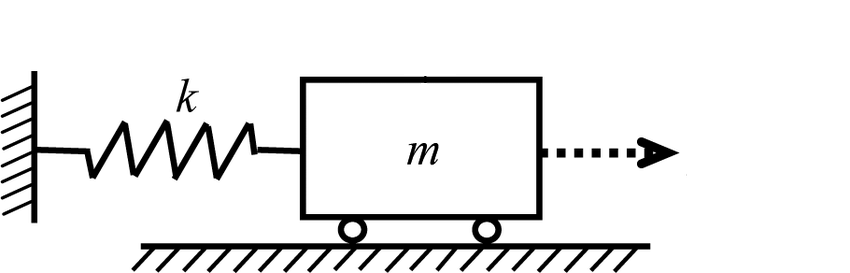
\includegraphics[width=.5\linewidth]{images/sdof-spring.png} \\
    Single degree of freedom spring
    \vspace{4ex}
  \end{minipage}%%
  \begin{minipage}[b]{0.5\linewidth}
    \centering
    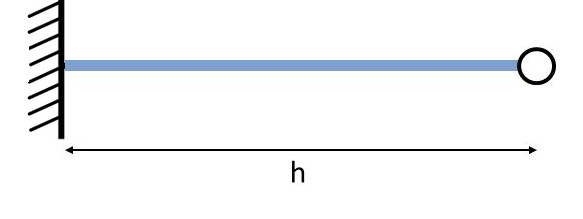
\includegraphics[width=.5\linewidth]{images/encastred.jpg} \\
    Fixed extremity 1D bar element
    \vspace{4ex}
  \end{minipage} 
  \begin{minipage}[b]{0.5\linewidth}
    \centering
    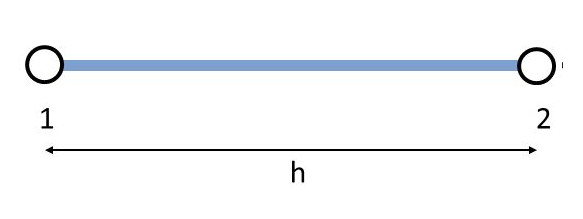
\includegraphics[width=.5\linewidth]{images/bar-element.jpg} \\
    1D bar element
    \vspace{4ex}
  \end{minipage}%% 
  \begin{minipage}[b]{0.5\linewidth}
    \centering
    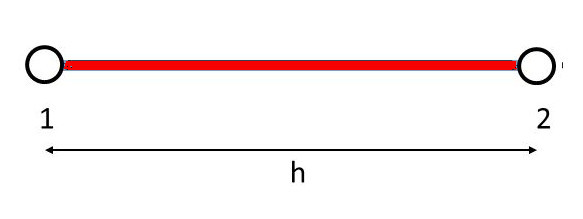
\includegraphics[width=.5\linewidth]{images/bar-element-pml.jpg} \\
    1D PML bar element
    \vspace{4ex}
  \end{minipage} 
\end{figure}
\end{frame}

\begin{frame}{SDOF spring}
\begin{itemize}
\item \underline{Single degree of freedom spring :}
\begin{figure}
\centering
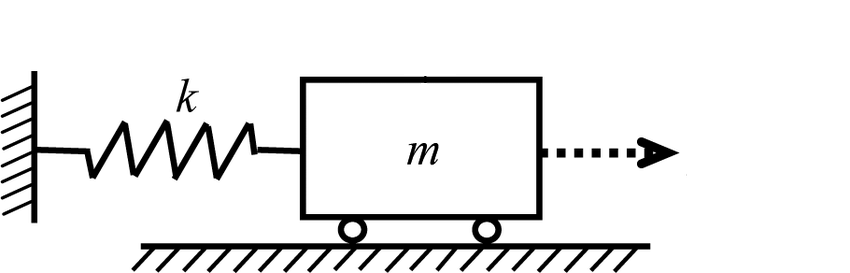
\includegraphics[width=0.5\linewidth]{images/sdof-spring.png}
\end{figure}
\end{itemize}
\end{frame}
\begin{frame}{SDOF spring: Implicit}
\begin{figure}[ht] 
  \label{ fig7} 
  \begin{minipage}[b]{0.5\linewidth}
    \centering
    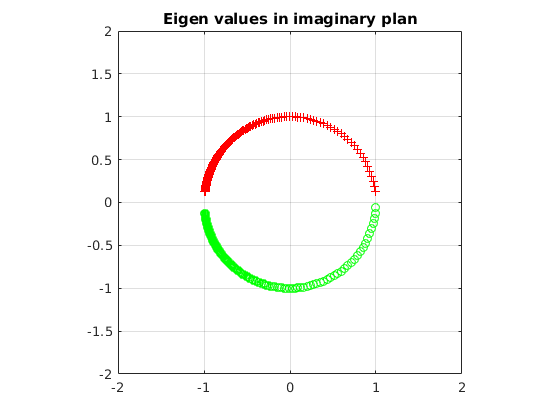
\includegraphics[scale=.35]{images/sdof-imp-1.png} \\

  \end{minipage}%%
  \begin{minipage}[b]{0.5\linewidth}
    \centering
    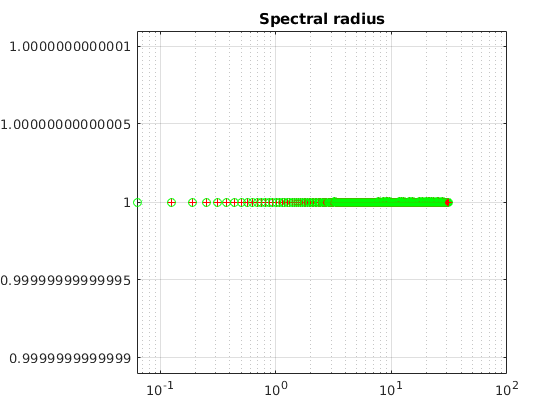
\includegraphics[scale=.35]{images/sdof-imp-2.png} \\
  \end{minipage} 
  \begin{minipage}[b]{0.5\linewidth}
    \centering
    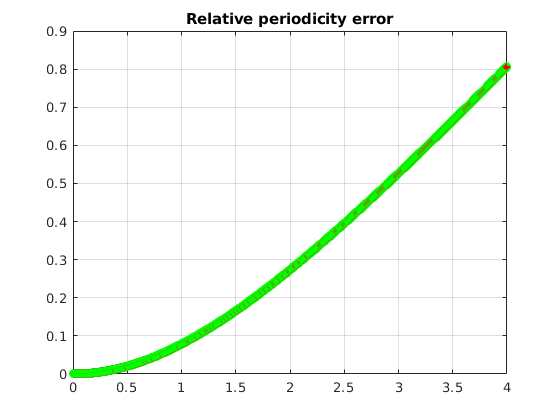
\includegraphics[scale=.35]{images/sdof-imp-3.png} \\

  \end{minipage}%% 
  \begin{minipage}[b]{0.5\linewidth}
    \centering
    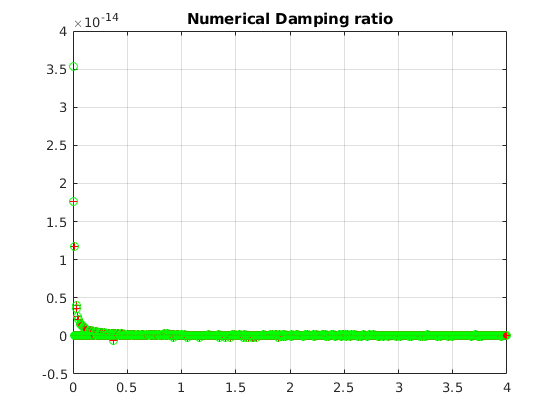
\includegraphics[scale=.35]{images/sdof-imp-4.png} \\

  \end{minipage} 
\end{figure}
\end{frame}

\begin{frame}{SDOF spring: Explicit}
\begin{figure}[ht] 
  \label{ fig7} 
  \begin{minipage}[b]{0.5\linewidth}
    \centering
    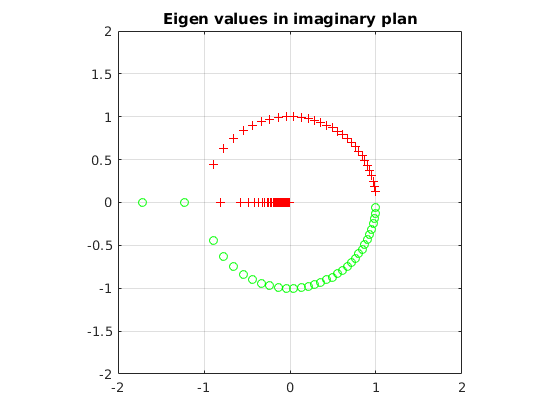
\includegraphics[scale=.35]{images/sdof-exp-1.png} \\

  \end{minipage}%%
  \begin{minipage}[b]{0.5\linewidth}
    \centering
    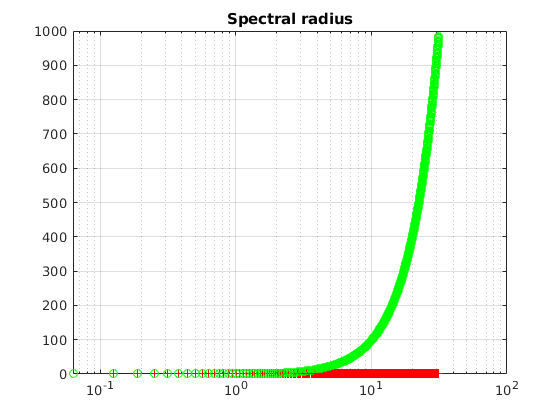
\includegraphics[scale=.35]{images/sdof-exp-2.png} \\
  \end{minipage} 
  \begin{minipage}[b]{0.5\linewidth}
    \centering
    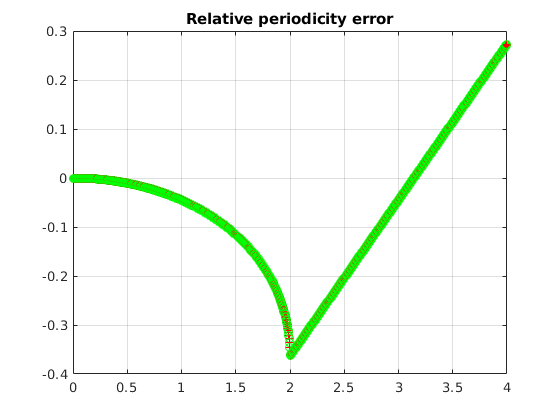
\includegraphics[scale=.35]{images/sdof-exp-3.png} \\

  \end{minipage}%% 
  \begin{minipage}[b]{0.5\linewidth}
    \centering
    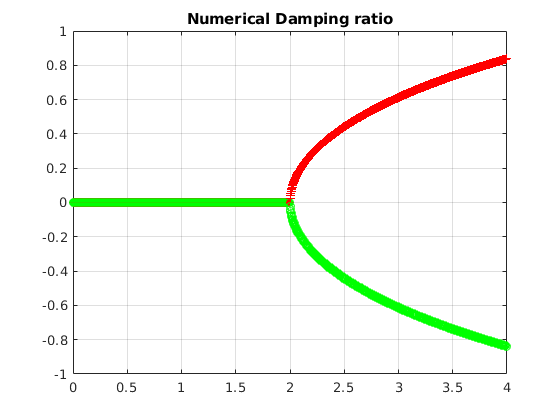
\includegraphics[scale=.35]{images/sdof-exp-4.png} \\

  \end{minipage} 
\end{figure}
\end{frame}

\begin{frame}{Encastred bar element}
\begin{itemize}
\item \underline{Encastred bar element :}
\begin{figure}
\centering
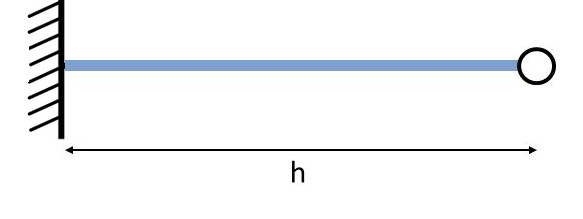
\includegraphics[width=0.5\linewidth]{images/encastred.jpg}
\end{figure}
\end{itemize}
\end{frame}

\begin{frame}{1D encastred element: Implicit}
\begin{figure}[ht] 
  \label{ fig7} 
  \begin{minipage}[b]{0.5\linewidth}
    \centering
    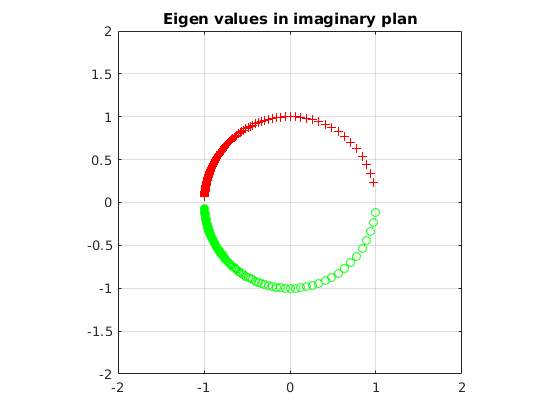
\includegraphics[scale=.35]{images/enc-imp-1.png} \\

  \end{minipage}%%
  \begin{minipage}[b]{0.5\linewidth}
    \centering
    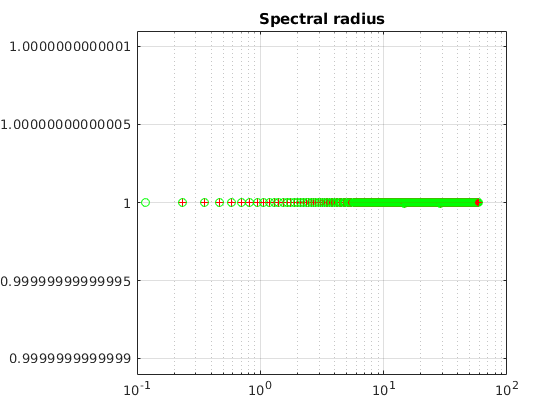
\includegraphics[scale=.35]{images/enc-imp-2.png} \\
  \end{minipage} 
  \begin{minipage}[b]{0.5\linewidth}
    \centering
    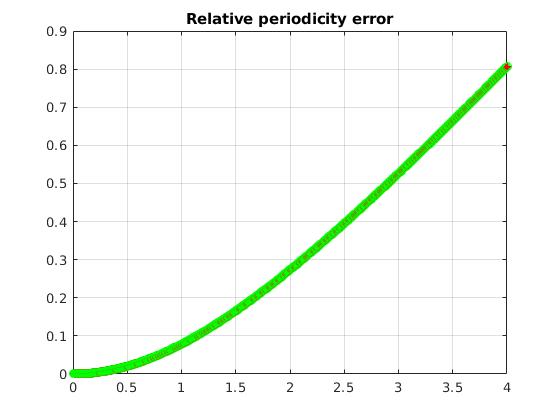
\includegraphics[scale=.35]{images/enc-imp-3.png} \\

  \end{minipage}%% 
  \begin{minipage}[b]{0.5\linewidth}
    \centering
    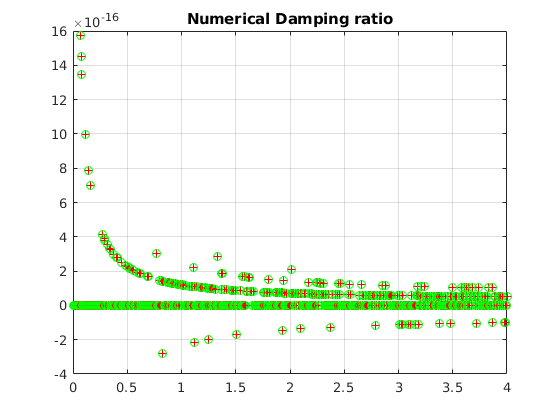
\includegraphics[scale=.35]{images/enc-imp-4.png} \\

  \end{minipage} 
\end{figure}
\end{frame}

\begin{frame}{1D Encastred element: Explicit}
\begin{figure}[ht] 
  \label{ fig7} 
  \begin{minipage}[b]{0.5\linewidth}
    \centering
    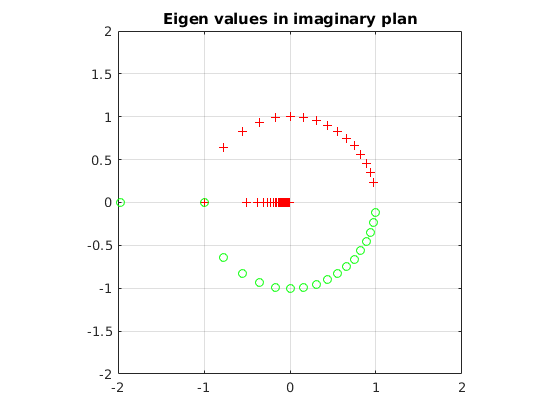
\includegraphics[scale=.35]{images/enc-exp-1.png} \\

  \end{minipage}%%
  \begin{minipage}[b]{0.5\linewidth}
    \centering
    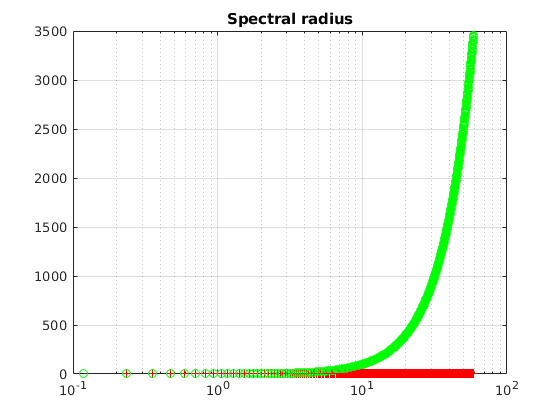
\includegraphics[scale=.35]{images/enc-exp-2.png} \\
  \end{minipage} 
  \begin{minipage}[b]{0.5\linewidth}
    \centering
    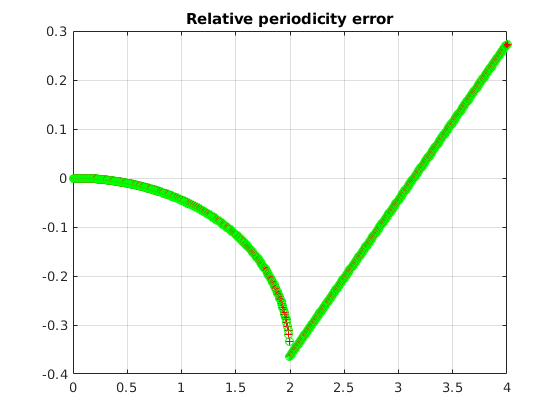
\includegraphics[scale=.35]{images/enc-exp-3.png} \\

  \end{minipage}%% 
  \begin{minipage}[b]{0.5\linewidth}
    \centering
    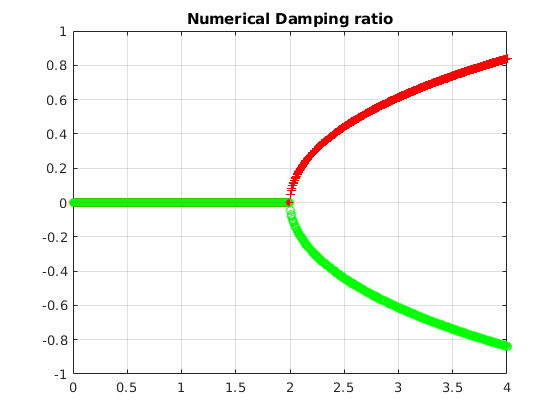
\includegraphics[scale=.35]{images/enc-exp-4.png} \\

  \end{minipage} 
\end{figure}
\end{frame}

\begin{frame}{1D bar element}
\begin{itemize}
\item \underline{1D bar element :}
\begin{figure}
\centering
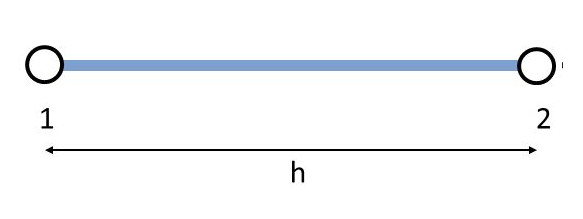
\includegraphics[width=0.5\linewidth]{images/bar-element.jpg}
\end{figure}
\end{itemize}
\end{frame}

\begin{frame}{1D bar element: Implicit}
\begin{figure}[ht] 
  \label{ fig7} 
  \begin{minipage}[b]{0.5\linewidth}
    \centering
    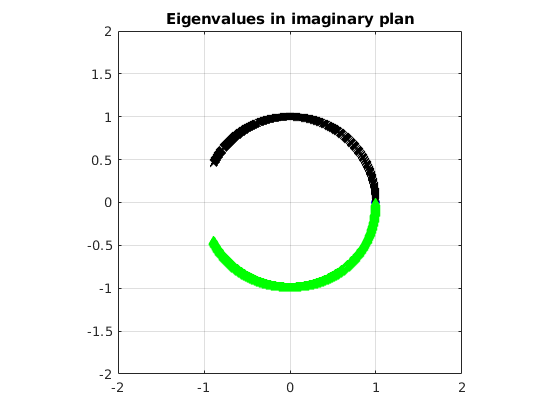
\includegraphics[scale=.35]{images/bar-imp-1.png} \\

  \end{minipage}%%
  \begin{minipage}[b]{0.5\linewidth}
    \centering
    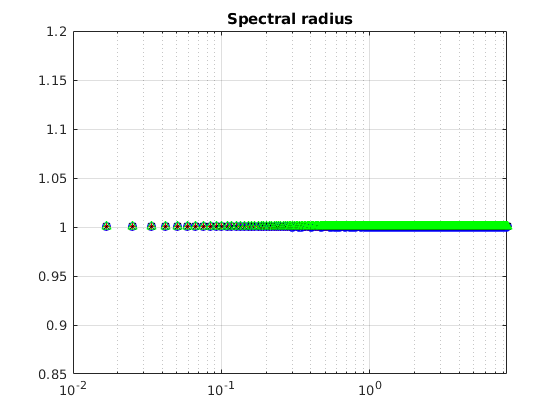
\includegraphics[scale=.35]{images/bar-imp-2.png} \\
  \end{minipage} 
  \begin{minipage}[b]{0.5\linewidth}
    \centering
    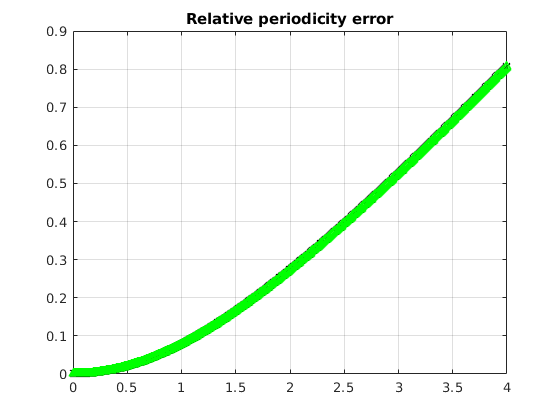
\includegraphics[scale=.35]{images/bar-imp-3.png} \\

  \end{minipage}%% 
  \begin{minipage}[b]{0.5\linewidth}
    \centering
    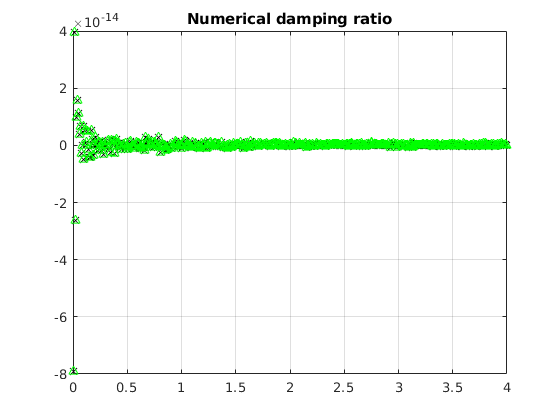
\includegraphics[scale=.35]{images/bar-imp-4.png} \\

  \end{minipage} 
\end{figure}
\end{frame}

\begin{frame}{1D bar element: Explicit}
\begin{figure}[ht] 
  \label{ fig7} 
  \begin{minipage}[b]{0.5\linewidth}
    \centering
    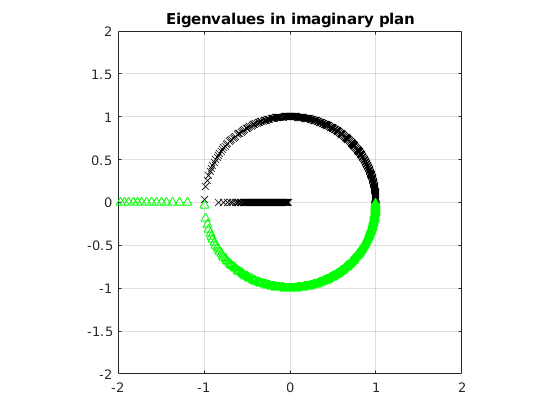
\includegraphics[scale=.35]{images/bar-exp-1.png} \\

  \end{minipage}%%
  \begin{minipage}[b]{0.5\linewidth}
    \centering
    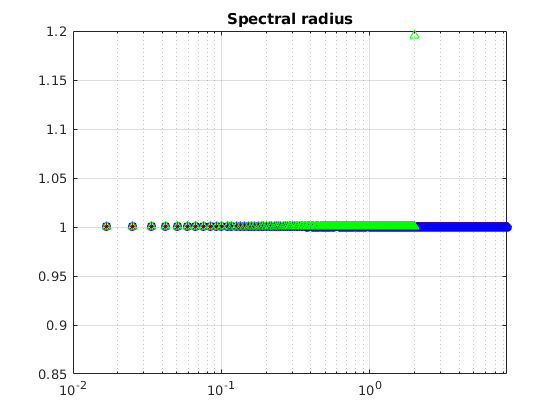
\includegraphics[scale=.35]{images/bar-exp-2.png} \\
  \end{minipage} 
  \begin{minipage}[b]{0.5\linewidth}
    \centering
    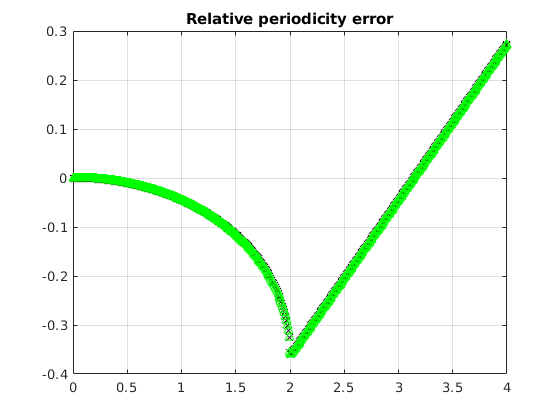
\includegraphics[scale=.35]{images/bar-exp-3.png} \\

  \end{minipage}%% 
  \begin{minipage}[b]{0.5\linewidth}
    \centering
    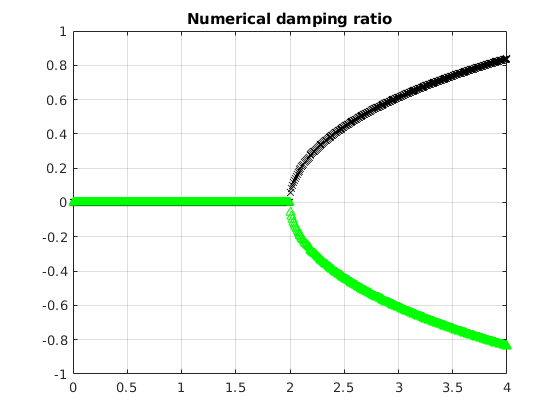
\includegraphics[scale=.35]{images/bar-exp-4.png} \\

  \end{minipage} 
\end{figure}
\end{frame}


\begin{frame}{1D PML bar element}
\begin{itemize}
\item \underline{1D PML bar element :}
\begin{figure}
\centering
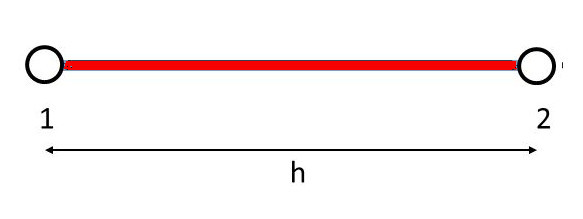
\includegraphics[width=0.5\linewidth]{images/bar-element-pml.jpg}
\end{figure}
\end{itemize}
\end{frame}

\begin{frame}{1D PML bar element: Implicit}
\begin{figure}[ht] 
  \label{ fig7} 
  \begin{minipage}[b]{0.5\linewidth}
    \centering
    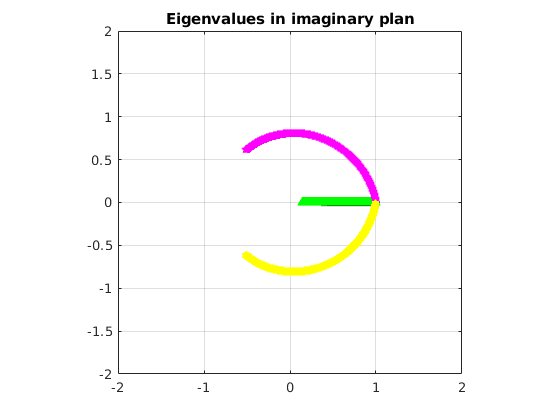
\includegraphics[scale=.35]{images/pml1d-imp-1.png} \\

  \end{minipage}%%
  \begin{minipage}[b]{0.5\linewidth}
    \centering
    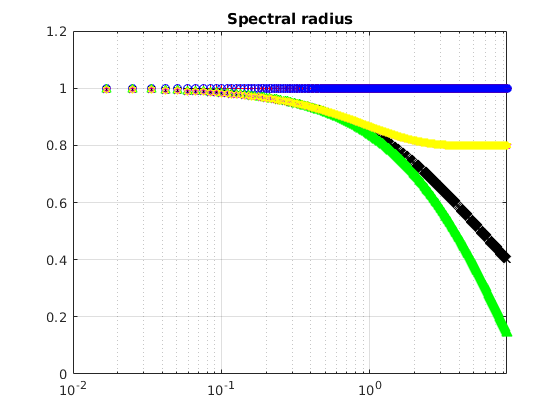
\includegraphics[scale=.35]{images/pml1d-imp-2.png} \\
  \end{minipage} 
  \begin{minipage}[b]{0.5\linewidth}
    \centering
    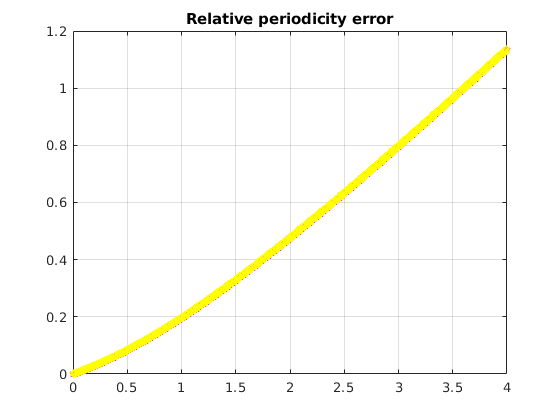
\includegraphics[scale=.35]{images/pml1d-imp-3.png} \\

  \end{minipage}%% 
  \begin{minipage}[b]{0.5\linewidth}
    \centering
    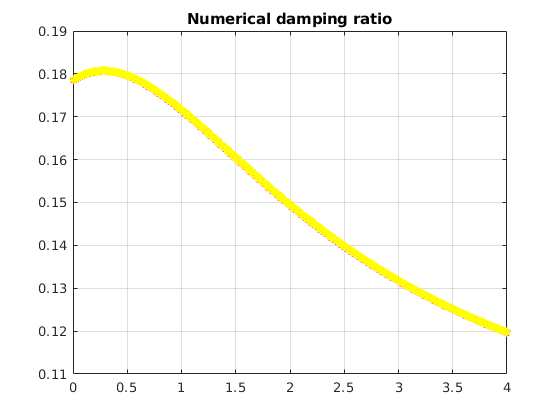
\includegraphics[scale=.35]{images/pml1d-imp-4.png} \\

  \end{minipage} 
\end{figure}
\end{frame}

\begin{frame}{1D PML bar element: Explicit}
\begin{figure}[ht] 
  \label{ fig7} 
  \begin{minipage}[b]{0.5\linewidth}
    \centering
    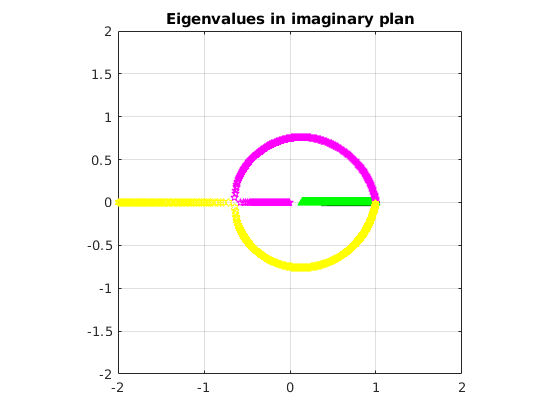
\includegraphics[scale=.35]{images/pml1d-exp-1.png} \\

  \end{minipage}%%
  \begin{minipage}[b]{0.5\linewidth}
    \centering
    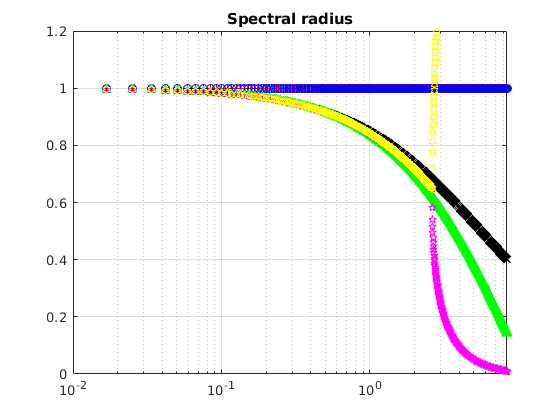
\includegraphics[scale=.35]{images/pml1d-exp-2.png} \\
  \end{minipage} 
  \begin{minipage}[b]{0.5\linewidth}
    \centering
    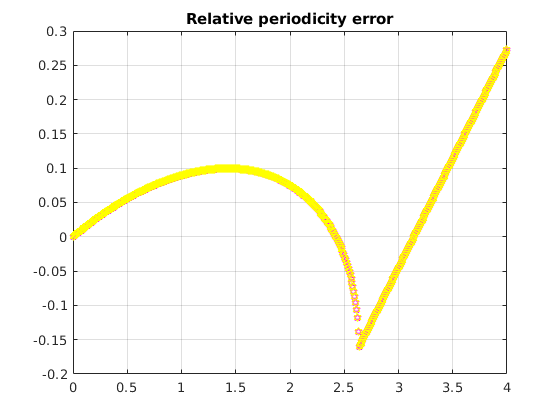
\includegraphics[scale=.35]{images/pml1d-exp-3.png} \\

  \end{minipage}%% 
  \begin{minipage}[b]{0.5\linewidth}
    \centering
    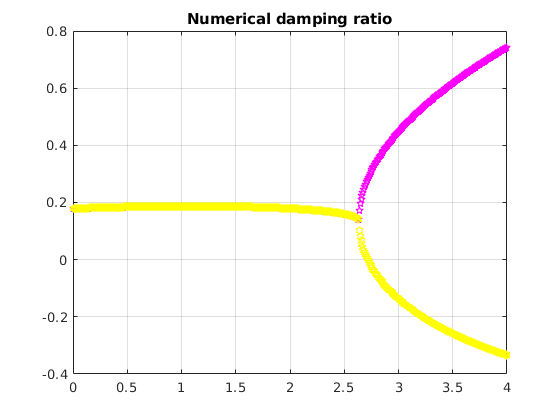
\includegraphics[scale=.35]{images/pml1d-exp-4.png} \\

  \end{minipage} 
\end{figure}
\end{frame}

\section{2D stability}
\begin{frame}{2D element stability}
\begin{itemize}
\item \underline{2D linear 4-noded element :}
\begin{figure}
\centering
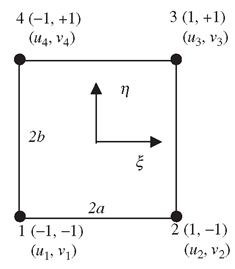
\includegraphics[width=0.4\linewidth]{images/square2d.png}
\end{figure}
\end{itemize}
\end{frame}

\begin{frame}{2D element: Implicit}
\begin{figure}[ht] 
  \label{ fig7} 
  \begin{minipage}[b]{0.5\linewidth}
    \centering
    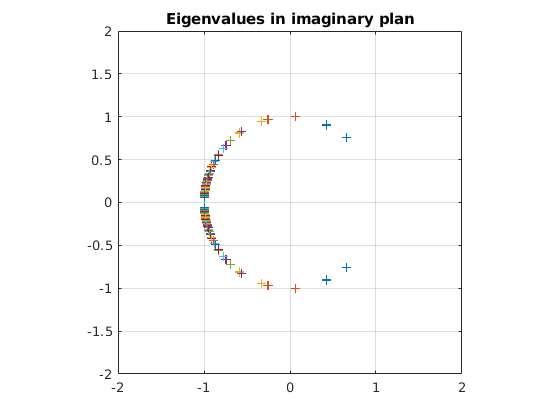
\includegraphics[scale=.35]{images/2D-imp-1.png} \\

  \end{minipage}%%
  \begin{minipage}[b]{0.5\linewidth}
    \centering
    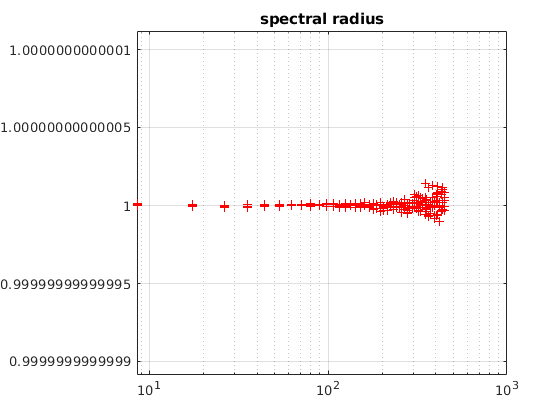
\includegraphics[scale=.35]{images/2D-imp-2.png} \\
  \end{minipage} 
  \begin{minipage}[b]{0.5\linewidth}
    \centering
    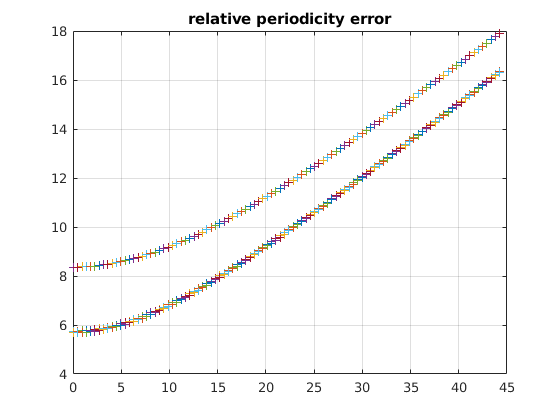
\includegraphics[scale=.35]{images/2D-imp-3.png} \\

  \end{minipage}%% 
  \begin{minipage}[b]{0.5\linewidth}
    \centering
    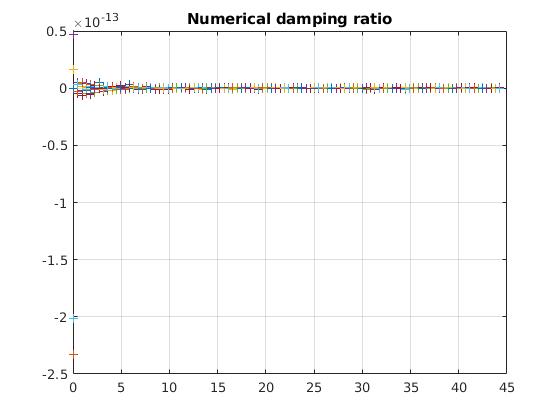
\includegraphics[scale=.35]{images/2D-imp-4.png} \\

  \end{minipage} 
\end{figure}
\end{frame}

\begin{frame}{2D element: Explicit}
\begin{figure}[ht] 
  \label{ fig7} 
  \begin{minipage}[b]{0.5\linewidth}
    \centering
    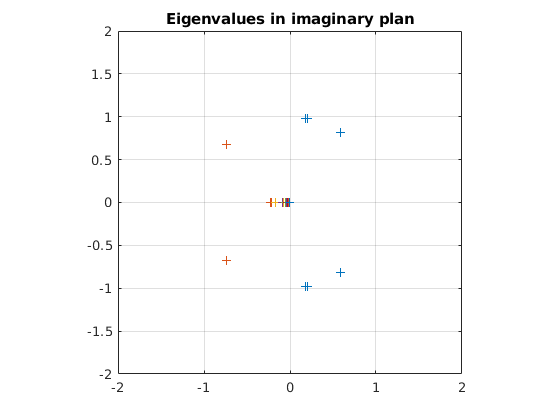
\includegraphics[scale=.35]{images/2D-exp-1.png} \\

  \end{minipage}%%
  \begin{minipage}[b]{0.5\linewidth}
    \centering
    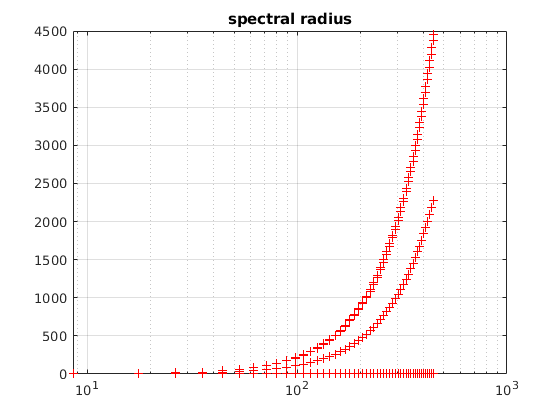
\includegraphics[scale=.35]{images/2D-exp-2.png} \\
  \end{minipage} 
  \begin{minipage}[b]{0.5\linewidth}
    \centering
    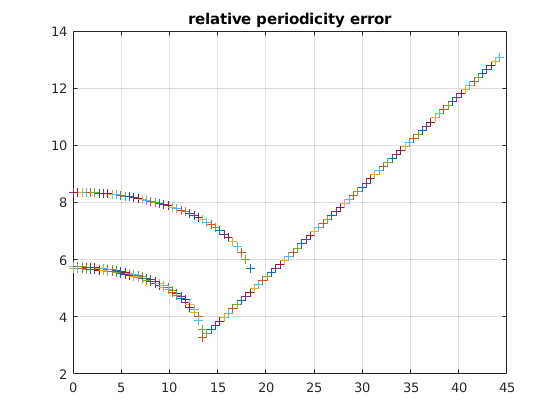
\includegraphics[scale=.35]{images/2D-exp-3.png} \\
  \end{minipage}%% 
  \begin{minipage}[b]{0.5\linewidth}
    \centering
    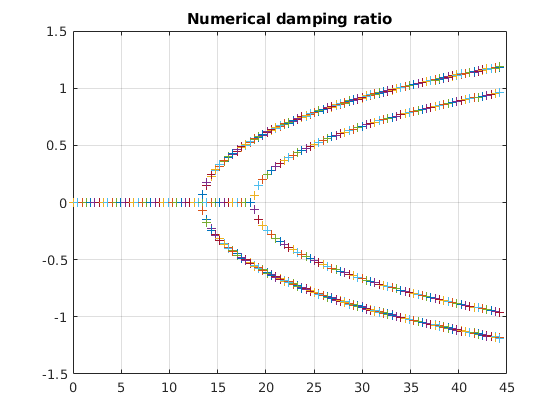
\includegraphics[scale=.35]{images/2D-exp-4.png} \\
  \end{minipage} 
\end{figure}
\end{frame}

\begin{frame}{2D element: Implicit}
\begin{figure}[ht] 
  \label{ fig7} 
  \begin{minipage}[b]{0.5\linewidth}
    \centering
    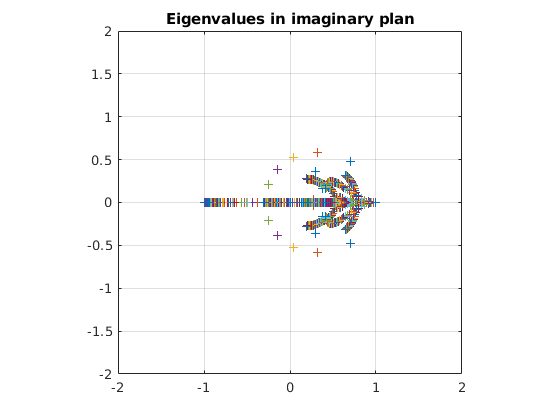
\includegraphics[scale=.4]{images/2Dpml-imp-1.png} \\

  \end{minipage}%%
  \begin{minipage}[b]{0.5\linewidth}
    \centering
    \includegraphics[scale=.4]{images/2Dpml-imp-2.png} \\
  \end{minipage} 

\end{figure}
\end{frame}

\begin{frame}{2D element: Explicit}
\begin{figure}[ht] 
  \label{ fig7} 
  \begin{minipage}[b]{0.5\linewidth}
    \centering
    \includegraphics[scale=.4]{images/2Dpml-exp-1.png} \\

  \end{minipage}%%
  \begin{minipage}[b]{0.5\linewidth}
    \centering
    \includegraphics[scale=.4]{images/2Dpml-exp-2.png} \\
  \end{minipage} 

\end{figure}
\end{frame}